\chapter[Partial Results]{Partial Results}

\section[Results]{Results}

The project has been successful so far, with the website being developed while the scripts were created and tested. This already creates a graphical installer, that will run in most linux distributions, for all the cataloged games developed with SDL 1.

\subsection[The Building Scripts]{The Building Scripts}

The building scripts were tested against half of the 16 available games. Table \ref{tab:script_games} shows which games were tested and the results of them. It was a success, because all the installers were created correctly for all of them (both GUI and \textit{.deb}). For some games, even with the correct compilation, they wouldn't run as expected, due to logical errors in their source code.

\begin{table}[h!]
\centering
\caption{Scripts results}
\label{tab:script_games}
\begin{tabular}{lcccc}
\hline
\textbf{Game} & \multicolumn{1}{l}{\textbf{Compiles?}} & \multicolumn{1}{l}{\textbf{.deb}} & \multicolumn{1}{l}{\textbf{QT}} & \multicolumn{1}{l}{\textbf{Runs?}} \\ \hline
Ankhnowledge & y & y & y & y \\
Post War & y & y & y & y \\
Jack the Janitor & y & y & y & y \\
Emperor vs Aliens & y & y & y & y \\
Ninja Siege & y & y & y & y \\
Space monkeys & y & y & y & n* \\
War of the Nets & y & y & y & n \\
Travelling Will & y & y & y & y \\ \hline
\end{tabular}
\end{table}

The game \textit{Space Monkeys} compiled correctly, however upon running it, the user couldn't do anything and the screens weren't precisely rendered. \textit{War of the Nets}, even compiling without errors, had a segmentation fault after a few seconds with the game open.

The building scripts are very similar, the only difference is that one builds games for SDL2 while the other uses SDL 1 (and their respective libraries). They work by cloning the repository and copying the required files to use CMake as seen in Algorithm \ref{alg:sdl}. This is the tool that actually compiles and builds everything. Because CMake generates a lot of files that are only used while it's running, professor Edson made a few more scripts to separate everything into folders and generate the installers.

\begin{algorithm}[h!]
\caption{Algorithm to build the games}
\label{alg:sdl}
\algblock[Name]{Start}{End}
\begin{algorithmic}
\Start
\State {$project \gets $} \Call{init}{$url,branch$} \Comment{Clone repository and set the project}
\State \Call{copy\_files}{$default, project$} \Comment{Copy templates}
\State {$project_{media\_dir} \gets $} \Call{find\_media}{}\Comment{Find the media folder}
\State {$project_{source\_dir} \gets $} \Call{find\_source}{}\Comment{Find the source folder and \textit{.cpp} files}
\State \Call{replace\_info}{$default, project$} \Comment{Replace template defaults}
\State \Call{rename}{$default, project$} \Comment{Rename some files}
\State \Call{build}{$project$} \Comment{Call the build script}
\State \Call{create\_installers}{$project$} \Comment{Create the installers}
\End
\end{algorithmic}
\end{algorithm}

% rep.copy_files()
% rep.find_media()
% rep.find_source()
% rep.replace_info()
% rep.rename()
% rep.build()

A major concern when making this script was its generality. It should run successfully with as many games as possible, requiring only a few tweaks in the source code or folder structure of the repository, if any. Starting with \textit{Jack the Janitor}, the example Professor Edson had made first, the  building script assumed a lot of things, mostly due to my inexperiencewith games and the folder structure adopted by the students. For example, in the initial versions, I thought all the \textit{.cpp} files would always be in a folder called \textit{src}. Another assumption was that all media would be in a \textit{media} folder.

Both of them proved me wrong as more games were tested, but were fairly easy to fix and keep the algorithm generic. For both folders, I had to modify the script to look for directories that would have similar names to those I thought were the rule. For example, \textit{source} instead of just \textit{src}, and \textit{resources}, \textit{res} and \textit{sound} instead of just \textit{media}. Even though this doesn't find all possible names, it follows a pattern found in most folder structures and all of the projects tested so far.

Another big premise was that all games would have their main file named \textit{main.cpp}. Even in repositories with Portuguese file names, it never occurred to me that anyone would name those files in any other way. However, a few games, specially \textit{Traveling Will} proved me wrong. Here, again, there was the option of looking for files named with similar words to \textit{main}, but this was a terrible option in this case, because the file could have \textit{any} name. Even if I looked for \textit{principal.cpp} that would not guarantee anything. Another option was parsing all the source files looking for the main function, but that would slow down the building process and would be error prone. Because there were so many options, I decided to keep it looking for \textit{main.cpp}, even if it required to manually change the repository.

\subsection[Platform]{Platform}

The website as of now allows an administrator to upload a game, with its respective information, like supported platform, related media, and installers.
The administrator has to manually add everything, since developers to all the game information, as seen in Figures \ref{fig:include_game1}. Figure \ref{fig:admin_home} shows the home page with all the administrator choices.

\begin{figure}[h!]
\centering
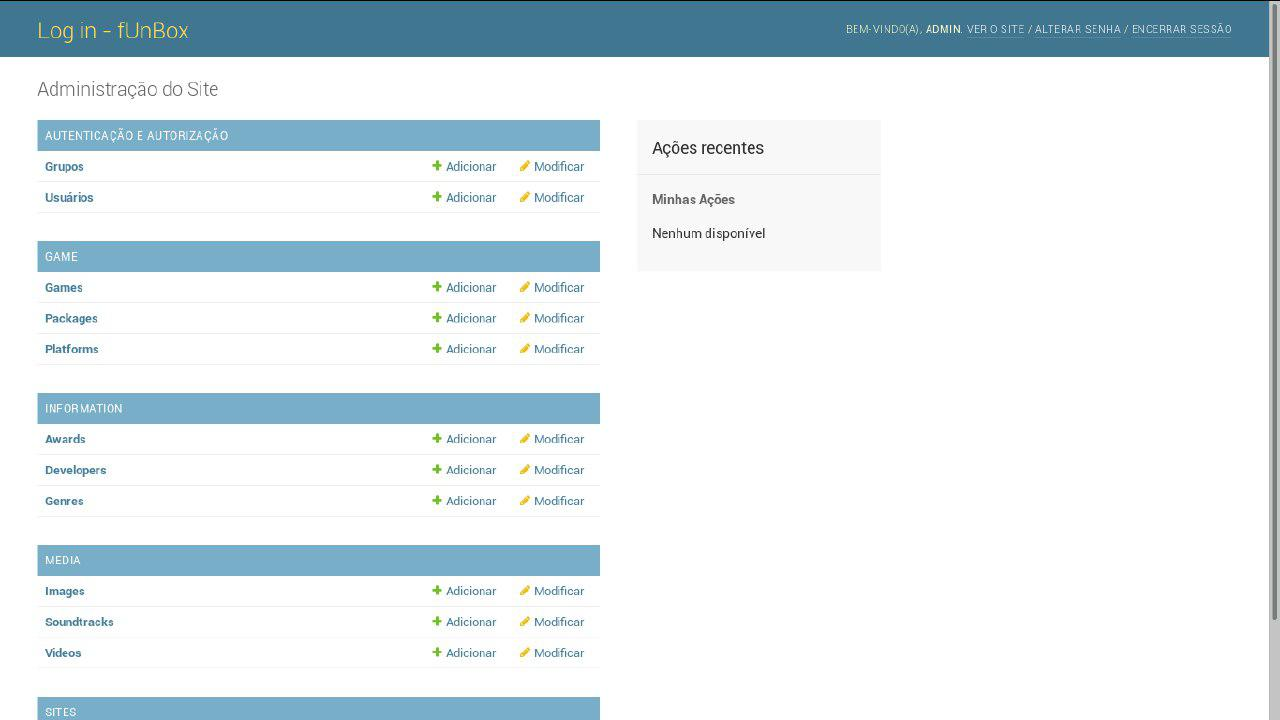
\includegraphics[width=\textwidth,height=\textheight,keepaspectratio]{admin_home_page}
\caption{Administrator home page}
\label{fig:admin_home}
\end{figure}

\begin{figure}[h!]
\centering
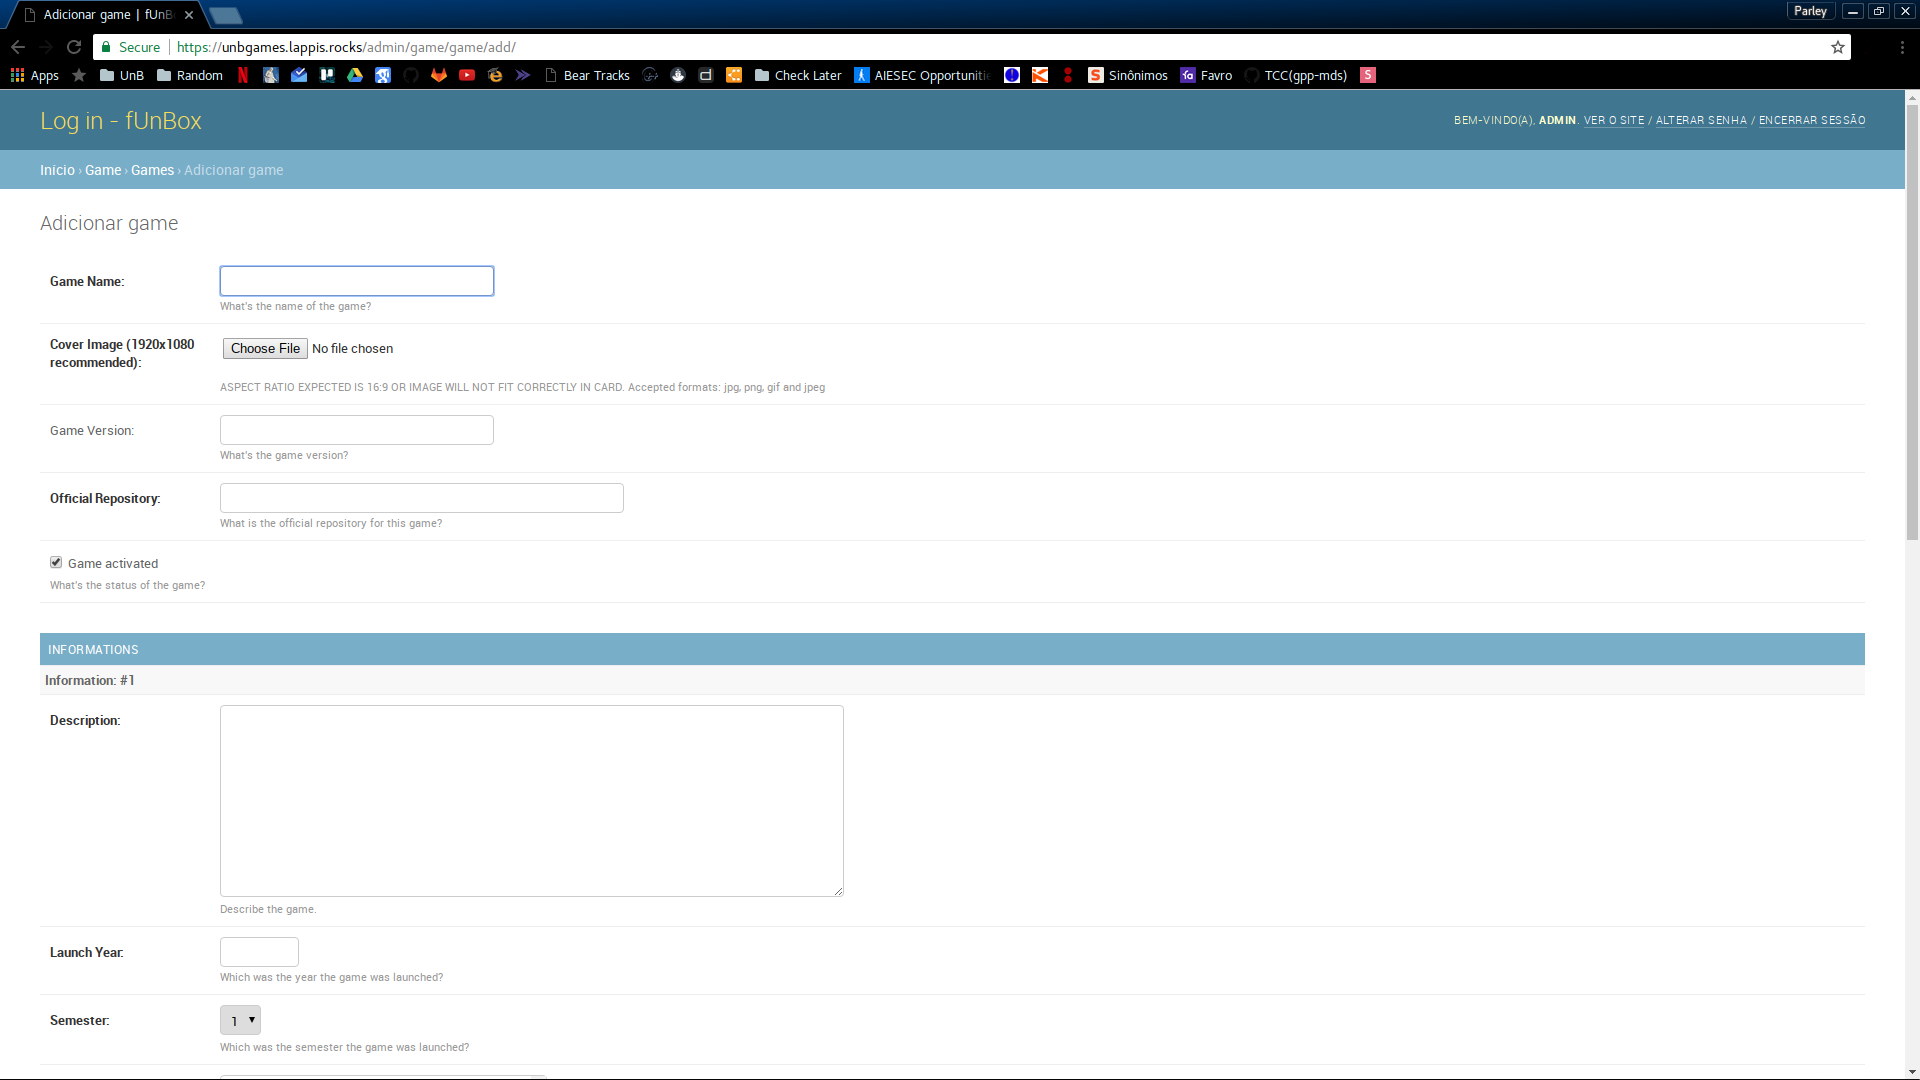
\includegraphics[width=\textwidth,height=\textheight,keepaspectratio]{include_game1}
\caption{Include new game}
\label{fig:include_game1}
\end{figure}

The general public can see a list of the available games. By choosing one, it's possible to see its information, download it for the available Operating Systems or comment using a Facebook account, as shown in Figures \ref{fig:game_list} and \ref{fig:game_detail}

\begin{figure}[h!]
\centering
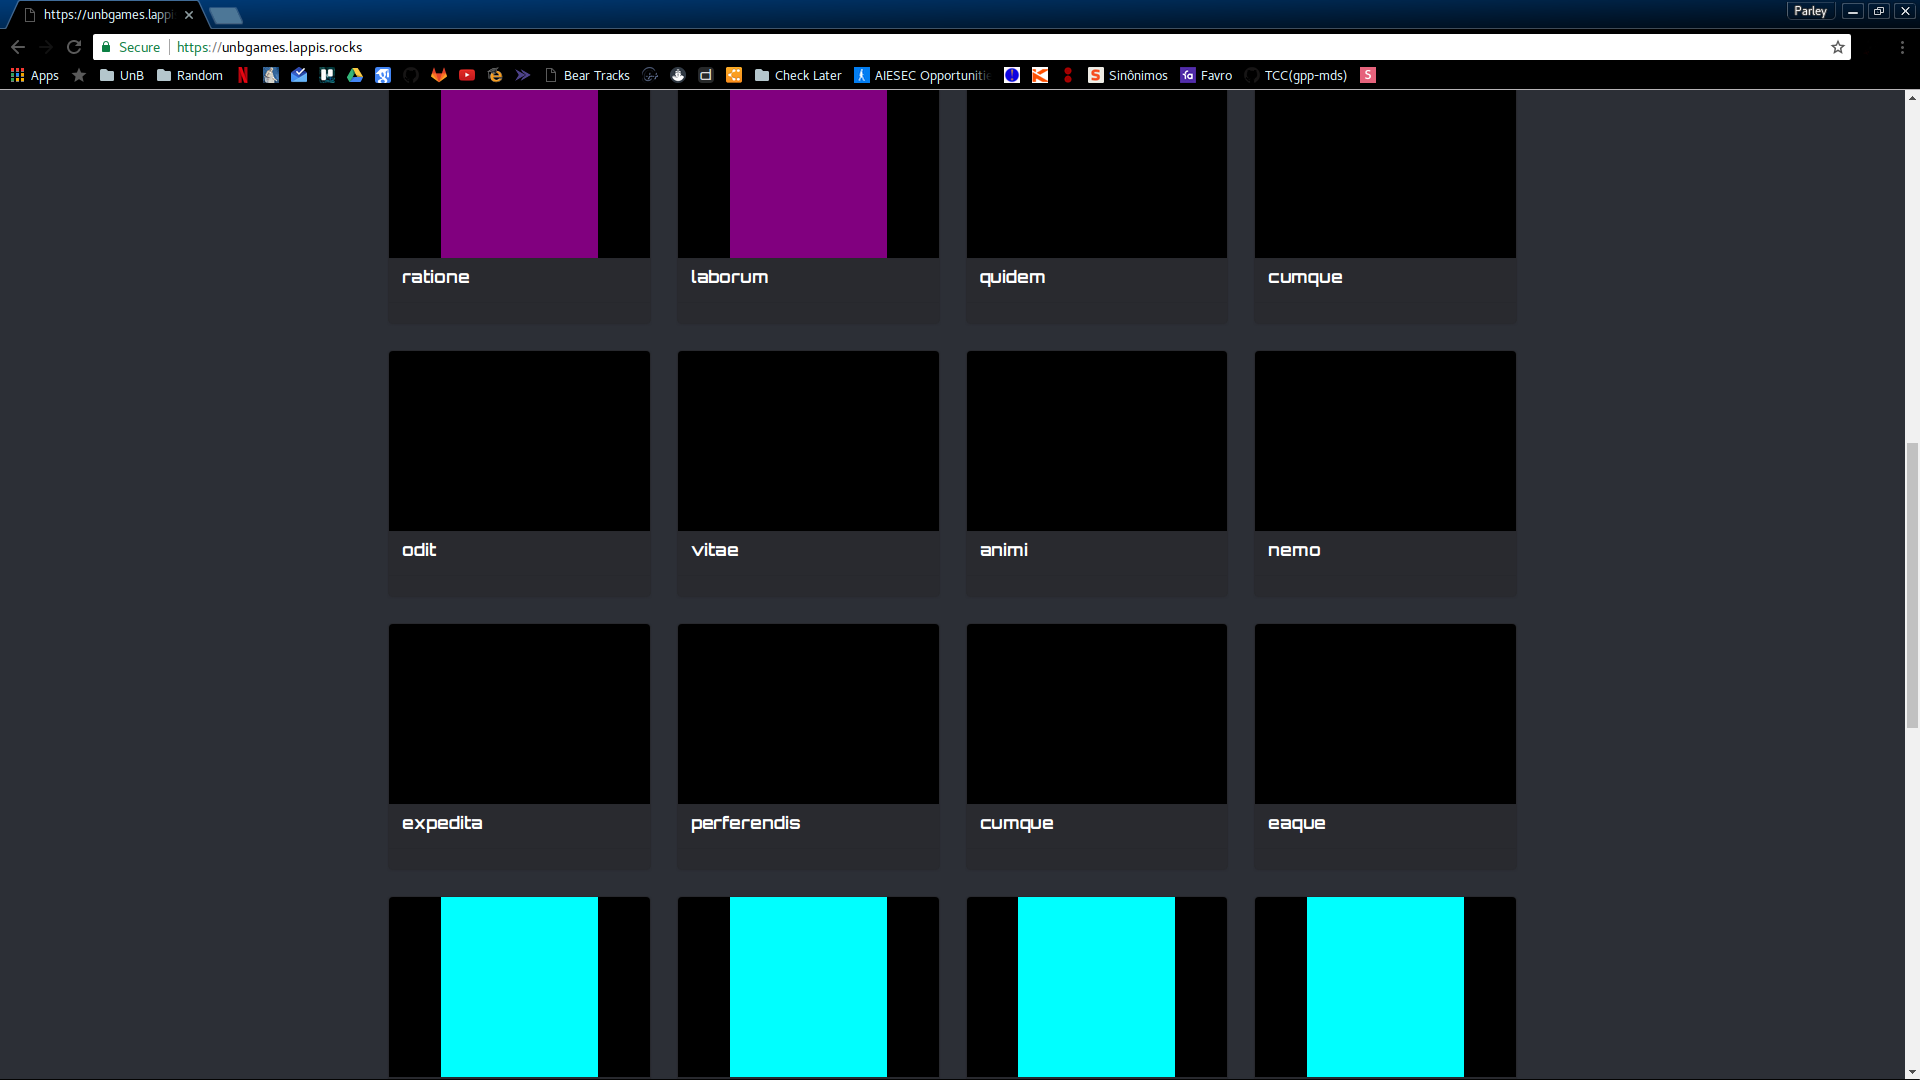
\includegraphics[width=\textwidth,height=\textheight,keepaspectratio]{game_list}
\caption{Game list}
\label{fig:game_list}
\end{figure}


\begin{figure}[h!]
\centering
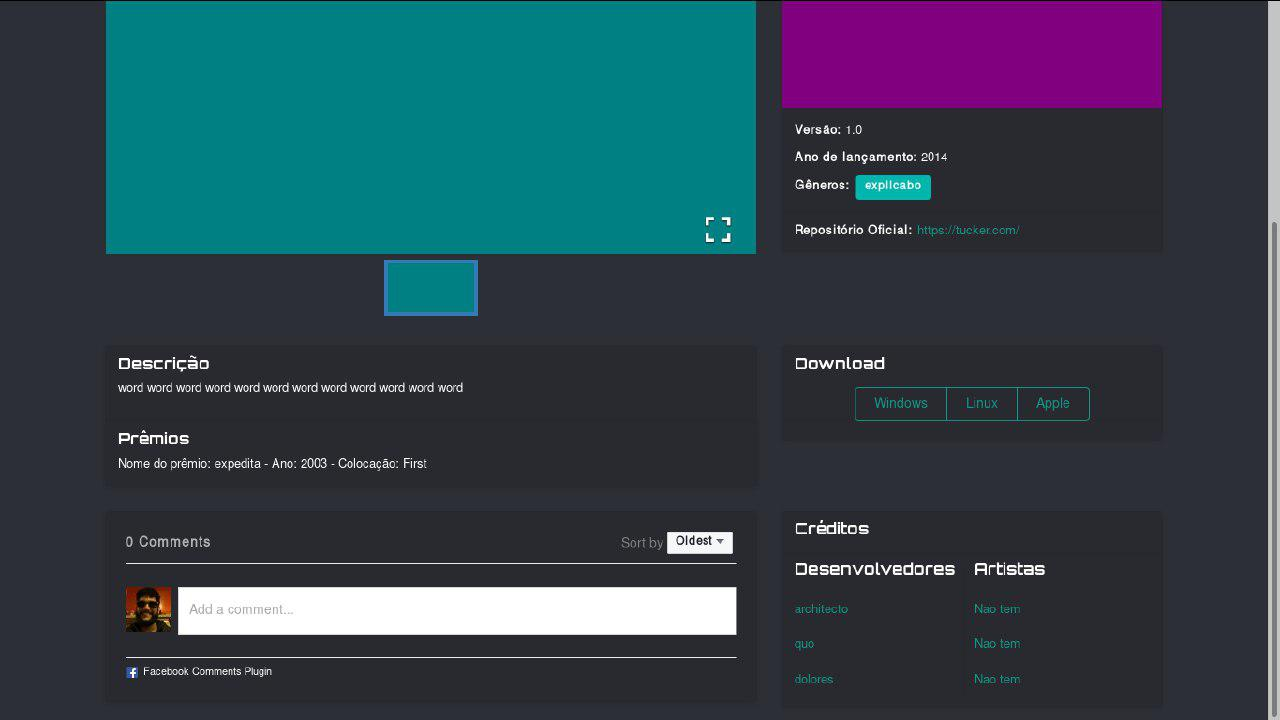
\includegraphics[width=\textwidth,height=\textheight,keepaspectratio]{game_detail}
\caption{Game detail}
\label{fig:game_detail}
\end{figure}

\section[Future Work]{Future Work}

For the next months it is expected to have the script for the SDL 2 projects finished with support for Windows and MacOS.

Another goal is to have the website running the script automatically when a user links their GitHub repository to the system.


\subsection[Schedule]{Schedule}

The following activities will be developed in the remaining time of the project. They are summarized in Figure \ref{fig:schedule}

\begin{itemize}
\item \textbf{Literature Review} - Review what the literature has on packaging, CMake, game development.
\item \textbf{Add Lua support} - Some of the games have lua as a dependency library that also needs to go in the final package..
\item \textbf{Add other Linux distros support} - Generate at least \textit{.rpm} packages.
\item \textbf{Add MacOS support} - Create install packages for Mac (Apple Systems).
\item \textbf{Add Windows support} - Make a installer (\textit{.exe}) to run on Windows 10 (maybe with some backwards compatibility if possible).
\item \textbf{Integrate to platform} - Run the scripts though a request on the website
\item \textbf{Integrate to GitHub} - Let users upload games thought GitHub hooks and read game information from there.
\item \textbf{Add Darcy's games} - Look for games developed in Darcy Ribeiro campus and test the script on them.
\item \textbf{Code refactoring} - Integrate scripts (SDL 1 and 2), make them more generic and efficient.
\item \textbf{Final adjustments} - Make minor improvements and fixes.
\item \textbf{Write Report} - Report progress and results.
\end{itemize}

\begin{figure}[h!]
\centering
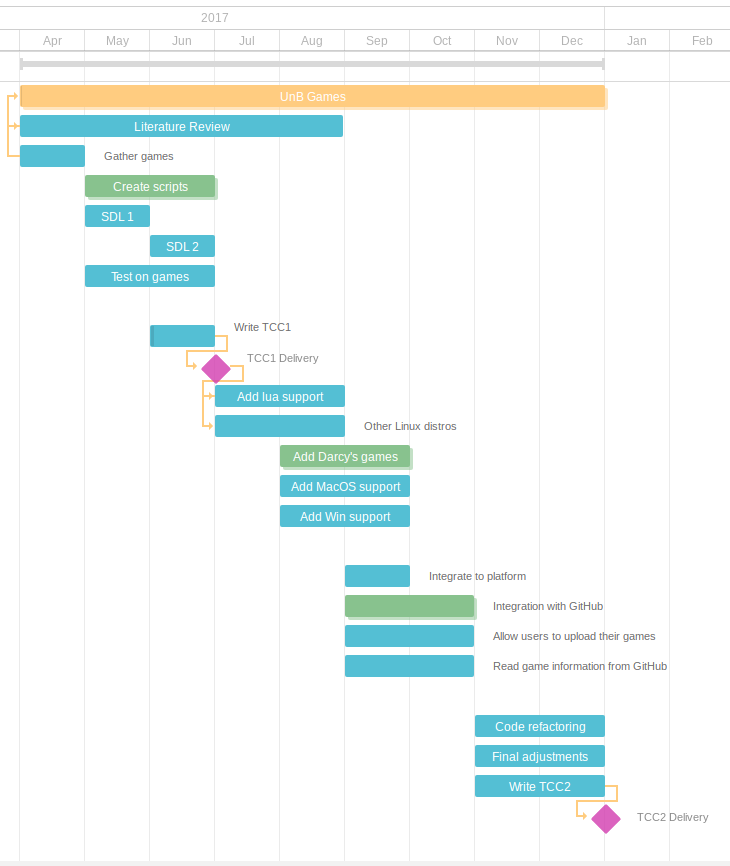
\includegraphics[width=\textwidth,height=\textheight,keepaspectratio]{gantt_chart}
\caption{Project Schedule}
\label{fig:schedule}
\end{figure}

% \begin{table}[h!]
% \centering
% \caption{Project Schedule}
% \label{tab:schedule}
% \begin{tabular}{|l|c|c|c|c|c|c|c|c|c|}
% \hline
% \textbf{Task} & \multicolumn{1}{l|}{\textbf{Apr}} & \multicolumn{1}{l|}{\textbf{May}} & \multicolumn{1}{l|}{\textbf{Jun}} & \multicolumn{1}{l|}{\textbf{Jul}} & \multicolumn{1}{l|}{\textbf{Ago}} & \multicolumn{1}{l|}{\textbf{Sep}} & \multicolumn{1}{l|}{\textbf{Oct}} & \multicolumn{1}{l|}{\textbf{Nov}} & \multicolumn{1}{l|}{\textbf{Dec}} \\ \hline
% Literature Review & x & x & x & x & x &  &  &  &  \\ \hline
% Add Lua support &  &  &  & x & x &  &  &  &  \\ \hline
% Add other distros support &  &  &  & x & x &  &  &  &  \\ \hline
% Add MacOS support &  &  &  &  & x & x &  &  &  \\ \hline
% Add Windows support &  &  &  &  & x & x &  &  &  \\ \hline
% Integrate to website &  &  &  &  & x & x &  &  &  \\ \hline
% Add Darcy's games &  &  &  &  &  & x & x &  &  \\ \hline
% Code refactoring &  &  &  &  &  &  & x & x &  \\ \hline
% Final adjustments &  &  &  &  &  &  &  & x & x \\ \hline
% Write Report &  &  & x &  &  &  &  & x & x \\ \hline
% \end{tabular}
% \end{table}
